% THIS IS SIGPROC-SP.TEX - VERSION 3.1
% WORKS WITH V3.2SP OF ACM_PROC_ARTICLE-SP.CLS
% APRIL 2009
%
% It is an example file showing how to use the 'acm_proc_article-sp.cls' V3.2SP
% LaTeX2e document class file for Conference Proceedings submissions.
% ----------------------------------------------------------------------------------------------------------------
% This .tex file (and associated .cls V3.2SP) *DOES NOT* produce:
%       1) The Permission Statement
%       2) The Conference (location) Info information
%       3) The Copyright Line with ACM data
%       4) Page numbering
% ---------------------------------------------------------------------------------------------------------------
% It is an example which *does* use the .bib file (from which the .bbl file
% is produced).
% REMEMBER HOWEVER: After having produced the .bbl file,
% and prior to final submission,
% you need to 'insert'  your .bbl file into your source .tex file so as to provide
% ONE 'self-contained' source file.
%
% Questions regarding SIGS should be sent to
% Adrienne Griscti ---> griscti@acm.org
%
% Questions/suggestions regarding the guidelines, .tex and .cls files, etc. to
% Gerald Murray ---> murray@hq.acm.org
%
% For tracking purposes - this is V3.1SP - APRIL 2009

\documentclass{acm_proc_article-sp}

\begin{document}

\title{A Sample {\ttlit ACM} SIG Proceedings Paper in LaTeX
Format\titlenote{(Does NOT produce the permission block, copyright information nor page numbering). For use with ACM\_PROC\_ARTICLE-SP.CLS. Supported by ACM.}}
\subtitle{[Extended Abstract]
\titlenote{A full version of this paper is available as
\textit{Author's Guide to Preparing ACM SIG Proceedings Using
\LaTeX$2_\epsilon$\ and BibTeX} at
\texttt{www.acm.org/eaddress.htm}}}
%
% You need the command \numberofauthors to handle the 'placement
% and alignment' of the authors beneath the title.
%
% For aesthetic reasons, we recommend 'three authors at a time'
% i.e. three 'name/affiliation blocks' be placed beneath the title.
%
% NOTE: You are NOT restricted in how many 'rows' of
% "name/affiliations" may appear. We just ask that you restrict
% the number of 'columns' to three.
%
% Because of the available 'opening page real-estate'
% we ask you to refrain from putting more than six authors
% (two rows with three columns) beneath the article title.
% More than six makes the first-page appear very cluttered indeed.
%
% Use the \alignauthor commands to handle the names
% and affiliations for an 'aesthetic maximum' of six authors.
% Add names, affiliations, addresses for
% the seventh etc. author(s) as the argument for the
% \additionalauthors command.
% These 'additional authors' will be output/set for you
% without further effort on your part as the last section in
% the body of your article BEFORE References or any Appendices.

\numberofauthors{8} %  in this sample file, there are a *total*
% of EIGHT authors. SIX appear on the 'first-page' (for formatting
% reasons) and the remaining two appear in the \additionalauthors section.
%
\author{
% You can go ahead and credit any number of authors here,
% e.g. one 'row of three' or two rows (consisting of one row of three
% and a second row of one, two or three).
%
% The command \alignauthor (no curly braces needed) should
% precede each author name, affiliation/snail-mail address and
% e-mail address. Additionally, tag each line of
% affiliation/address with \affaddr, and tag the
% e-mail address with \email.
%
% 1st. author
\alignauthor
Ben Trovato\titlenote{Dr.~Trovato insisted his name be first.}\\
       \affaddr{Institute for Clarity in Documentation}\\
       \affaddr{1932 Wallamaloo Lane}\\
       \affaddr{Wallamaloo, New Zealand}\\
       \email{trovato@corporation.com}
% 2nd. author
\alignauthor
G.K.M. Tobin\titlenote{The secretary disavows
any knowledge of this author's actions.}\\
       \affaddr{Institute for Clarity in Documentation}\\
       \affaddr{P.O. Box 1212}\\
       \affaddr{Dublin, Ohio 43017-6221}\\
       \email{webmaster@marysville-ohio.com}
% 3rd. author
\alignauthor Lars Th{\o}rv{\"a}ld\titlenote{This author is the
one who did all the really hard work.}\\
       \affaddr{The Th{\o}rv{\"a}ld Group}\\
       \affaddr{1 Th{\o}rv{\"a}ld Circle}\\
       \affaddr{Hekla, Iceland}\\
       \email{larst@affiliation.org}
\and  % use '\and' if you need 'another row' of author names
% 4th. author
\alignauthor Lawrence P. Leipuner\\
       \affaddr{Brookhaven Laboratories}\\
       \affaddr{Brookhaven National Lab}\\
       \affaddr{P.O. Box 5000}\\
       \email{lleipuner@researchlabs.org}
% 5th. author
\alignauthor Sean Fogarty\\
       \affaddr{NASA Ames Research Center}\\
       \affaddr{Moffett Field}\\
       \affaddr{California 94035}\\
       \email{fogartys@amesres.org}
% 6th. author
\alignauthor Charles Palmer\\
       \affaddr{Palmer Research Laboratories}\\
       \affaddr{8600 Datapoint Drive}\\
       \affaddr{San Antonio, Texas 78229}\\
       \email{cpalmer@prl.com}
}
% There's nothing stopping you putting the seventh, eighth, etc.
% author on the opening page (as the 'third row') but we ask,
% for aesthetic reasons that you place these 'additional authors'
% in the \additional authors block, viz.
\additionalauthors{Additional authors: John Smith (The Th{\o}rv{\"a}ld Group,
email: {\texttt{jsmith@affiliation.org}}) and Julius P.~Kumquat
(The Kumquat Consortium, email: {\texttt{jpkumquat@consortium.net}}).}
\date{30 July 1999}
% Just remember to make sure that the TOTAL number of authors
% is the number that will appear on the first page PLUS the
% number that will appear in the \additionalauthors section.

\maketitle
\begin{abstract}
% !TeX root = 
Distributed matrix computations are becoming more and more ubiquitous in the world. Algorithms for problems like Noisy Matrix Factorization have applications in many areas such as the recommender systems used by Netflix, Movielens, and many others. These algorithms have many parameters and settings that must be tweaked in order to achieve specified error or time bounds. Many operators simply manually tweak the parameters to get whatever behavior they require, however this is clearly both expensive and prone to error. In this work we propose a general system to automate parameter choice for distributed matrix computations. We implement our optimizer and use it to optimize the division parameter in Divide-Factor-Combine (DFC), a recently-developed matrix factorization algorithm. We find that running the algorithm with the optimizer-chosen parameters yields the best behavior of any manually chosen parameter setting, regardless of any constraints imposed on the time or error of the computation.
\end{abstract}

% A category with the (minimum) three required fields
\category{H.4}{Information Systems Applications}{Miscellaneous}
%A category including the fourth, optional field follows...
\category{D.2.8}{Software Engineering}{Metrics}[complexity measures, performance measures]

\terms{Theory}

\keywords{ACM proceedings, \LaTeX, text tagging} % NOT required for Proceedings

\section{Introduction}
% !TeX root = ../AdaptiveSeedingSTOC.tex
With the rising public use of the Internet in modern times, companies 
such as Google or Facebook are gathering increasingly massive amounts 
of data. These companies often want to leverage their huge databases to 
learn and predict hidden information. For example, Netflix utilizes user 
ratings to improve their recommendation system, which finds new and 
interesting movies for their users to watch. In order to properly 
process these mountains of information, researchers have invested
considerable into the development of distributed algorithms for 
various machine learning tasks. For example, the Noisy Matrix Factorization 
problem is at the core of many online recommendation systems, and is
also useful in concisely representing data. Recently, a strongly parallel 
algorithm for this problem called Divide-Factor-Combine was developed 
at UC Berkeley\cite{MTJ13}. 

\subsection{The Problem}
These machine learning algorithms often take in many parameters, and
to achieve the best results, the input parameters must be optimized for
each specific application. In addition, the use of parallelism and the
nature of convergent algorithms creates a tradeoff between time, accuracy,
and the number of processors or machines tasked with the computation. 
On the one hand, too much parallelism can cause the algorithm to lose 
error guarantees and perform inadequately. On the other hand, too 
little parallelism can make the computation take an unacceptably long 
amount of time. On top of that, monetary budgets may restrict the number
of machines or processors one is willing to dedicate to the task, limiting
the capacity for parallelism. The objectives of minimizing both the error 
and time of the computation within a monetary budget are obviously 
in conflict.

Further, different users may have different requirements over these 
domains. In the case of an online recommendation system, as more 
customers buy or rate products, it is necessary to rerun the machine 
learning task in order to ensure relevant and current recommendations. 
Here the user may have some time budget describing how long he can wait 
for the machine learning algorithm to run, and would want to minimize 
the prediction error of the algorithm subject to this budget. On the other
hand, a genome scientist who has collected partial genetic data 
across many organisms may care more about maximizing the accuracy of the
phenotype prediction, but have a much more relaxed time budget. 

Either extensive empirical tests or an operator who is extremely 
familiar with both the dataset and the algorithm is required in order 
to achieve optimal results for a particular problem instance. In addition,
optimized parallelization choices might meet time budgets on one particular
architecture but fail on another, as communication times and machine
speeds can vary drastically. For these reasons, it is very desirable 
to have an automated process that can pick settings that meet budgets
reliably, and solve the problem optimally within budget constraints; such
an automated process could be architecture-independent, and adapt 
as the distribution of input data changes over time. 

\subsection{Our Contribution}
In this work we propose an optimizer for choosing parameter settings for 
distributed machine learning algorithms, in particular for distributed 
matrix computations. Given input data and user-specified budgets, our 
optimizer automatically chooses algorithm parameters to minimize either
time, error, or monetary expenditure while not going over-budget in any 
of these realms. The optimizer maintains a database of the parameter 
choices and empirical performance of previous jobs, and uses this stored 
information to choose optimal parameters for new incoming jobs.

Our optimizer has done quite well in tests, consistently performing as 
well as the best possible manual choice of parameters. Our preliminary 
implementation currently optimizes the Divide-Factor-Combine algorithm 
for Noisy Matrix Factorization. Our tests were preformed on both synthetic 
and real-world data. Our synthetic data was in the form of Gaussian 
random matrices, and our real-world data was the Movielens10M 
dataset\footnote{\url{http://grouplens.org/datasets/movielens/}}. We have designed out optimizer to be general and easily 
extensible, and adding additional machine learning algorithms to our 
optimizer framework is the subject of ongoing work.


\section{Background}
\input{background.tex}

\section{Optimizer Design}
% !TeX root = 

When designing the optimizer, our goals were to provide a simple 
interface to the user and ensure architecture-independence. To meet the
objective of a simple user interface, the optimizer must be able to
make parameter choices based only on user-specified time, accuracy, and
monetary budget constraints. To meet
the objective of architecture-independence, the optimizer needs to gather
data about jobs run in its specific architecture context. Below,
we describe the design of the optimizer in pursuit of these goals. 

\subsection{Optimizer System Context}


\subsubsection{Interface to User}
The user's interface with the optimizer is simple: the user needs to
provide a problem instance for the job, constraints on the amount of
time and money that the job can spend and on the amount of error
that is acceptable for the output. The user also specifies $X$, the 
parameter to be optimized (currently, $X$ can be total runtime, total
error, or amount of money spent).

The user can also specify whether to run the optimizer in {\em explore 
mode}, a mode suitable for high-variance data applications or if the 
optimizer is in the initial stages of learning a new 
distribution (see Section \ref{sec:explore}). 

Also, the user specifies which distribution the data comes from (by
distribution, we simply mean the source of the data, since data from
different sources may behave differently). Currently,
this is accomplished by having the user point the optimizer to the 
source of the learned data. When using the optimizer for the first 
couple of times, the user can input statistics from training on similarly
distributed data. There is also a more cursory mode available, in which
the optimizer runs a subproblem and obtains estimates for a wider 
variety of parameter settings (see Section \ref{sec:nodata}). In this 
mode, the user need not specify the distribution of the data. 

\subsubsection{Interface with Algorithm and Infrastructure}
Our optimizer relies on access to an already implemented distributed 
algorithm. The optimizer outputs the parameters that the algorithm 
should run with; in the current implementation this is limited to 
the number of processors and the number of iterations, although this
can be easily extended to algorithm-specific parameters (i.e. learning
rate). 
The algorithm itself is expected to communicate with the distributed
computation framework, although this too could be altered if necessary.

After the algorithm returns, the optimizer requires information about
the outcome of the job so that it can learn. We want to learn the error
and runtime as a function of the number of iterations and the number
of processors used. Because the input parameters are determined by the
optimizer (and thus already known to it), all the optimizer requires 
from the algorithm's output is the error and the runtime. In principle,
if there is an additional parameter over which one wishes to optimize
(say, for example, testing error in addition to training error),
additional information about the algorithm output must be stored. 

\subsection{Larnin'}

Our optimizer's parameter selection strategy is based on statistical 
data from prior runs. 
To ensure that the optimizer's choices are architecture-independent,
and to allow the optimizer to adapt to data from different distributions 
and to continually improve its predictions, our optimizer learns from
every job that it encounters. 




\subsection{Choosing Parameters}

\subsubsection{Choosing Parameters using Learned Data}
When given a problem instance with a particular budget, our optimizer
consults data from prior runs in order to select the algorithm 
parameters. 

\subsubsection{Choosing Parameters in the Absence of Data}
\label{sec:nodata}

Thus far, our described methods of parameter selection rely on a database
of information about previously completed jobs. However, when instances
from a new data distribution are initially run, there is no past data upon
which we can draw.

For this setting, we do the following: first, we run such a job for some
small number of iterations, in order to get some cursory data (this can
easily be modified as appropriate; we can run several small jobs, as the 
time budget allows). Then, we use this data to create estimates of the 
error, time to completion, and expenditure as a function of number of 
iterations and number of processors used.

From our empirical observations, the error is an exponential function of
the number of iterations, with an additive term which depends on the number
of processors:
\[
err(s,t) = A\cdot s + e^{-B\cdot t}.
\]
where $s$ is the number of processors and $t$ is the number of iterations, 
and $A$ and $B$ are unknown constants. The time to completion, at least 
in this method, we have observed to be a polynomial function of the 
number of processors:
\[
time(s,t) = \frac{t}{s^{C}}.
\]
where again $s$ is the number of processors, $t$ is the number of iterations, and $C$ is some unknown constant. This is essentially an application of 
Ahmdahl's Law, but for the application we chose to test on (DFC) the
serial time is negligible compared to the parallel time.

What we do in this case is try to fit the extant data from the small
cursory runs to these models, and then use these estimates to choose
the number of iterations and number of processors that optimize $X$ 
within the user's budget. In practice, our initial estimates are 
quite poor (see TODO). 

However, what matters is that the estimates of $X$ for different 
parameter settings are relatively accurate; that is, if the true value 
of $X$ will be better with parameter settings $p_1$ than with parameter
settings $p_2$, then the estimated one should be better as well.

\subsubsection{Explore Mode}
\label{sec:explore}
If the optimizer has access to few previous job outcomes, or if the data
comes from a very high-variance distribution, there is a risk that 
suboptimal parameter settings will be chosen again and again, simply 
because there was one very successful run with those settings, or because
the optimal settings are not known and the optimizer's estimated values
of $X$ are too high for other settings.

In order to prevent the optimizer from returning again and again to
these local optima, the optimizer is able to run in {\em explore mode}. 
In {\em explore mode}, randomization is
used to avoid local optima in parameter selection. Say that we have 
parameter settings $p_1, \ldots, p_m$ with estimated optimized values 
$x_1, \ldots, x_m$. Then the optimizer chooses the output parameters $P$ 
to be $p_i$ with probability
\[
\Pr[P = p_i] = \frac{\frac{1}{x_i}}{\sum_{j = 1}^m \frac{1}{x_j}}.
\]
This scheme has the property that if $\frac{x_i}{x_j} = \alpha$, 
then $\frac{\Pr[P = p_i]}{\Pr[P = p_j]} = \frac{1}{\alpha}$--that is, a 
particular parameter setting is chosen with probability proportional 
to its relative minimization of $X$.

In this way, the randomness guarantees that the optimizer explores the 
parameter space. Thus as the number of jobs encountered grows, 
the optimizer's data about the entire parameter space improves, and the
influence of outliers on parameter choice is subdued. 




\section{Divide-Factor-Combine}
For testing and evaluation of our optimizer we implemented several variants of the DFC (Divide-Factor-Combine) framework for distributed matrix completion, originally introduced in \cite{MTJ13}.

\subsection{DFC Framework Overview}
In this section we describe the matrix factorization problem that the DFC framework solves, and also outline the three main steps in the algorithm. 
\subsubsection{Problem Definition}
The DFC framework is used to solve the following well-studied noisy matrix completion problem: Let $A$ be an unknown $m\times n$ matrix of rank $r$, and assume $r<<m,n$. Next $A'$ is obtained by adding a small amount of noise to every entry of $A$. Finally, let $M$ be the matrix obtained by sampling a small fraction (e.g $10\%$) of the entries of $A'$, and setting all other entries to zero. We refer to $M$ as the matrix of revealed entries. The goal is then to find a low-rank matrix $B$ that is a good approximation of the original matrix $A$, using only the matrix $M$. The standard method of finding such a low rank matrix $B$ is to find a low-rank factorization $B=UV^T$ that agrees with $M$ on all of its non-zero entries.

A version of this problem is actually solved in practice by online movie-recommendation systems. Here the matrix has rows corresponding to users and columns corresponding to movies. The assumption that the matrix is low rank corresponds to the assumption that users movie preferences are only based on a relatively small number of factors (e.g. movie genre, movie length, user age etc). The matrix $M$ of revealed entries corresponds to the set of actual movie ratings that users have submitted.

\subsubsection{The DFC Algorithm}
The DFC framework for noisy matrix completion consists of three steps:
\begin{itemize}
\item \textbf{Divide} the input matrix $M$ column-wise into $k$ slices $\{M_1,M_2,...M_k\}$. More specifically, $M_i$ consists of $n/k$ columns from $M$ and concatenating all the $M_i$ gives the original matrix $M$. We call $k$ the \emph{division parameter} of DFC.
\item \textbf{Factor} each matrix $M_i$ as $U_i V_i^T$ on a separate processor using some base matrix factorization algorithm.
\item \textbf{Combine} the factorizations $U_iV_i^T$ into one large factorization $UV^T$ using some matrix column projection algorithm.
\end{itemize}
From this description it is clear that there are several significant choices to be made in the implementation of this framework. First, both the base factorization algorithm and the projection algorithm for the combine step must be chosen. Second, the parameter $k$ for determining the number of slices to cut the matrix into has an impact both on runtime and accuracy of the result.

\subsection{Base Factorization Algorithm Choices}
We implemented two base matrix factorization algorithms: Stochastic Gradient Descent (SGD) and Accelerated Proximal Gradient Descent (APG). Both algorithms seek to minimize some objective function which is a combination of the error of the approximation and the rank of the factorization.
\subsubsection{Stochastic Gradient Descent}
Let $\Omega$ be the set of indices for the revealed entries (i.e. non-zero entries) of the input matrix $M$. The objective function for the Stochastic Gradient Descent algorithm is given by:
\[
F(U,V,M) = \sum_{(i,j)\in \Omega} \left(M_{ij} - (UV^T)_{ij}\right)^2 + \mu (\| U\|^2_F  + \| V\|^2_F)
\]
where $\|U\|_F$ denotes the Frobenius norm of $U$ and $\mu$ is a parameter. Intuitively, the first term in the objective function penalizes errors in matching the revealed entries of $M$ and the second term is a regularization term to prevent over-fitting. The SGD algorithm uses standard gradient descent techniques to compute $\mbox{argmin}_{U,V} F(U,V,M)$. 

There are two important issues to note about the SGD algorithm. Firstly, the above minimization requires fixed choices for the dimensions of both $U$ and $V$. In particular, this means that we have to first decide on a rank $r$ for our factorization. Then we can run SGD to find a rank $r$ factorization that approximates $M$ well. The second issue is that the objective function $F(U,V,M)$ is not convex, so there can be local minima where the SGD algorithm gets stuck.

\subsubsection{Accelerated Proximal Gradient Descent}
We use the Accelerated Proximal Gradient Descent algorithm described in \cite{TY10}. The objective function for the APG algorithm is given by:
\[
F(U,V,M) = \sum_{(i,j)\in \Omega} \left(M_{ij} - (UV^T)_{ij}\right)^2 + \mu \| UV^T\|_*
\]
where $\|UV^T\|_*$ is the nuclear norm of $UV^T$. The key point here is that the nuclear norm is a convex relaxation of the rank. This means that the above objective in some sense tries to minimize both the error in matching the revealed entries of $M$, and some reasonable approximation of the rank of $B=UV^T$.

The algorithm has neither of the drawbacks of SGD. The user does not have to provide a guess for the rank, and the objective function is convex. Thus, the APG algorithm converges to a unique minimum, and there are theoretical guarantees on the convergence time.

\subsubsection{Base Algorithm Choice: APG}
We implemented both APG and SGD as described above, but it quickly became apparent that APG was superior for our purposes. The requirement that the user specify a rank for the factorization in SGD was a particularly large problem. First of all, having to specify a rank does not make a lot of sense when working with real-world data. For example, with a matrix of movie ratings it is not obvious apriori how many factors influence a user's movie preference. This is something that one would like the algorithm to determine automatically, as APG does.

The second issue is that choosing the target rank of the factorization adds another parameter to the algorithm. Our optimizer uses data about the parameter settings of previous tasks to automatically choose parameters for a new task. As a result, the number of previous examples we need to cover the whole parameter space is exponential in the total number of parameters. So any additional parameter (such as the rank parameter to APG) greatly increases the number of examples required for the optimizer to preform well.

The fact that the SGD objective function is not convex also causes multiple issues in our setting. We observed empirically that there was much more variance in the runtime and accuracy of SGD based on the starting point. Since the objective is not convex, we had to simply run SGD until the improvement at each iteration got small enough. Since there are several local minima, this can result in quite different run times even on matrices from the same distribution. 

In comparison, APG has theoretical guarantees on its convergence, and we empirically observed that running for a fixed number of iterations on matrices from the same distribution resulted in relatively small variation in both error and runtime. This small variation is critical to the success of our optimizer in predicting the error and runtime of new matrix factorization tasks based on previous runs.

\subsection{Matrix Projection Algorithm Choices}
We implemented two possible algorithms for the matrix projection that occurs in the combine step of DFC. The first was Column Projection and the second was Randomized Projection.

\subsubsection{Column Projection}
Given factorizations $(U_i,V_i)$ of each column slice $M_i$, the Column Projection algorithm simply projects each factorization $U_i V_i^T$ for $i \geq 2$ onto the column space of $U_1$. For each $i \geq 2$ this gives a new set of factorizations $U_1 \hat{V}_i^T$. Now we let $V^T$ be the  matrix obtained by the concatenation $[\hat{V}_1^T, \hat{V}_2^T..., \hat{V}_k^T]$. Then our final combined factorization is given by $U_1 V^T$.

Column Projection is very fast as it simply requires $k$ matrix projections. It does however rely on the assumption that the columns of $U_1$ span the column space of the full low-rank factorization of $M$. In situations where the size $n/k$ of a column slice is large relative to the rank of the factorization, this assumption is somewhat reasonable. However, there is still the risk that this projection method results in a small loss in accuracy due to the assumption.

\subsubsection{Randomized Projection}
The Randomized Projection algorithm we use was introduced by Halko et. al. in \cite{HMT10}. The algorithm is inspired by the Johnson-Lindenstrauss randomized method for metric embeddings. The algorithm involves sampling a random Guassian matrix and computing several QR factorizations. As a result, the algorithm is slower than the Column Projection algorithm. However, it has better theoretical guarantees on accuracy.

\subsubsection{Projection Algorithm Choice: Randomized Projection}
Despite the aforementioned tradeoffs in speed versus accuracy, we chose to use only the Randomized Projection algorithm. The reason for this was that it gave consistently better error than Column Projection, but the difference in runtime was very minimal. Further, the time take by the projection step in DFC is completely dominated by the time taken for the actual matrix factorizations. In particular, the projection time is less than $1\%$ of the time taken by the Factor step. As a result, accuracy at this step is more important than slight differences in run time. 

\section{Evaluation}
% !TeX root = ../AdaptiveSeedingSTOC.tex

In this section we evaluate the ability of the optimizer to optimize 
a single parameter in the DFC algorithm with respect to very simple 
utility functions and budgets. We test the optimizer on both synthetic 
and real-world datsets and conclude that most of the time it performs 
as well as the best manual parameter settings. 

\subsection{Methodology}

We evaluate the optimizer on both Gaussian Random matrices and the 
Movielens10M dataset 
(available at \url{http://grouplens.org/datasets/movielens/}). 
For each of the two datasets, we divided the available data 
into several partitions. For the random matrices we used five 
partitions, and this simply meant one matrix per partition. 
For the Movielens data (which is one enormous matrix), we 
partitioned the rows of the matrix into seven pieces (meaning, we 
subdivided the data into groups of users). 
This gave the two datasets a comparable number of nonzero entries 
per partition. 

After partitioning the data, we group the partitions into training 
data and testing data. We used all but one partition for both datasets 
as training data on which to run DFC computations. The optimizer was 
then fed the input and output profiles of these computations to use 
in its database. We used the final partition to test the predictions 
of the optimizer. 

Our goal was for the optimizer to automatically choose the degree 
of parallelism in the DFC algorithm, i.e. how much to slice the 
input matrix in the Divide step. We asked for the computations to 
be completed within a specified amount of time while minimizing the 
error, and DFC computations with manually-chosen parameters designed 
to meet these budgets were performed on this testing data, as well as 
a DFC computation with optimizer-chosen division. Error was computed 
using the Root Mean Square Error (RMSE) of the returned factorization 
compared to the revealed entries, and the time of a computation is 
defined as the maximum time of a slice computation plus the time 
it takes to finish the projection step of DFC.  

The evaluation metric we chose was, for each time budget, the error 
of the optimized parameters compared to the error of the \emph{best} 
run with manually-chosen parameters. We define the \emph{regret} 
of the optimizer on these instances as the average over the budgets 
of the percent difference in error of the optimized and manual parameters. 
We will see soon that the optimizer performs as well as the best parameter 
for every budget, even when that parameter changes depending on the 
budget. Finally, we performed cross-validation, i.e. training and 
testing was done with each of the partitions used as testing data, 
and we obtain very consistent results. 

We implemented the DFC algorithm in SparkR \cite{V13}, and the optimizer 
in Python. All of our tests were performed on the Amazon EC2 Cluster 
using medium instances. 

\subsection{Gaussian Random Matrices}
The first dataset we tested the optimizer on was a synthetic 
dataset containing many low rank randomly generated matrices. 
The matrices were generated according to the following procedure: 
\begin{enumerate}
\item Fix parameters $r$, $p$, and $\sigma^2$ which are the rank, 
percent of revealed entries, and the variance of the noise respectively.
\item Generate two $n \times r$ matrices ${\bf A}$ and ${\bf B}$ with 
entries drawn from $\mathcal{N}(0,1/\sqrt{r})$. 
\item Let ${\bf N}$ be an $n \times n$ matrix with ${\bf N}(i,j)$ drawn 
independently from $\mathcal{N}(0,\sigma^2)$. 
\item Define ${\bf M} = {\bf A}{\bf B}^T + {\bf N}$
\item Pick a uniform random subset $\Omega \subset [n] \times [n]$ 
with $|\Omega| = pn^2$, and let ${\bf M}_{\Omega}$ be the matrix such 
that ${\bf M}_{\Omega}(i,j) = {\bf M}$ for $(i,j) \in \Omega$ and 
unknown otherwise. 
\end{enumerate}
This procedure generates a noisy copy of a rank $r$ random matrix 
whose entries have unit variance and hides most of its entries. 
Now we can generate many of these matrices and by running a lot of 
DFC computations for training purposes, we can predict the behavior 
of DFC on these kinds of instances and thus automatically 
choose how much to divide the input. 

We generated five $4000 \times 4000$ matrices with 
\[(r,p,\sigma^2) = (10,.1,.01),\] 
and split the data into training/testing splits as mentioned 
in the previous section. Figure \ref{fig:4ktraintest} displays the 
results of one of the training/testing splits of the data. 
Each curve of the graph represents a choice of the division parameter 
in DFC. The first graph is the training data and we can empirically 
see that there are specific intersection points where the parameter 
choice should change. The second graph shows the error of DFC 
computations with manually chosen and optimized parameters. 
Each curve represents a specific choice of the division parameter, 
and the bold curve represents the choices made by the optimizer. 
We can see that the optimizer consistently chooses whichever division 
optimizes the error within the specified time budget. 

Table \ref{fig:4kCrossTable} summarizes the results of each of the 
training/testing splits. Averaged over all these splits, the optimized 
parameter choices perform within $1\%$ over the minimal error, 
and always meeting the budget.

\begin{table}
\label{fig:4kCrossTable}
\begin{center}
    \begin{tabular}{| p{2.2cm} | p{2.2cm} | p{2.2cm} |}
    \hline
    Testing Set & \% Over Optimal Error & \% Over Time Budget \\ \hline
    1 & 0.03\% & -11.7\% \\ \hline
    2 & 0.50\% & -13.1\% \\ \hline
    3 & 0.42\% & -13.8\% \\ \hline
    4 & 0.94\% & -16.1\% \\ \hline
    5 & 0.53\% & -12.4\% \\ \hline
    \end{tabular}
\end{center}
\caption{Average regret and time for k-fold cross-validation of optimizer run on five Gaussian random matrices of dimension 4000 by 4000. Percentages are in relationship to best possible error and time budget respectively.}
\end{table}

\begin{figure*}
\label{fig:4ktraintest}
	\begin{subfigure}[b]{.45\textwidth}
\begin{center}
		\fbox{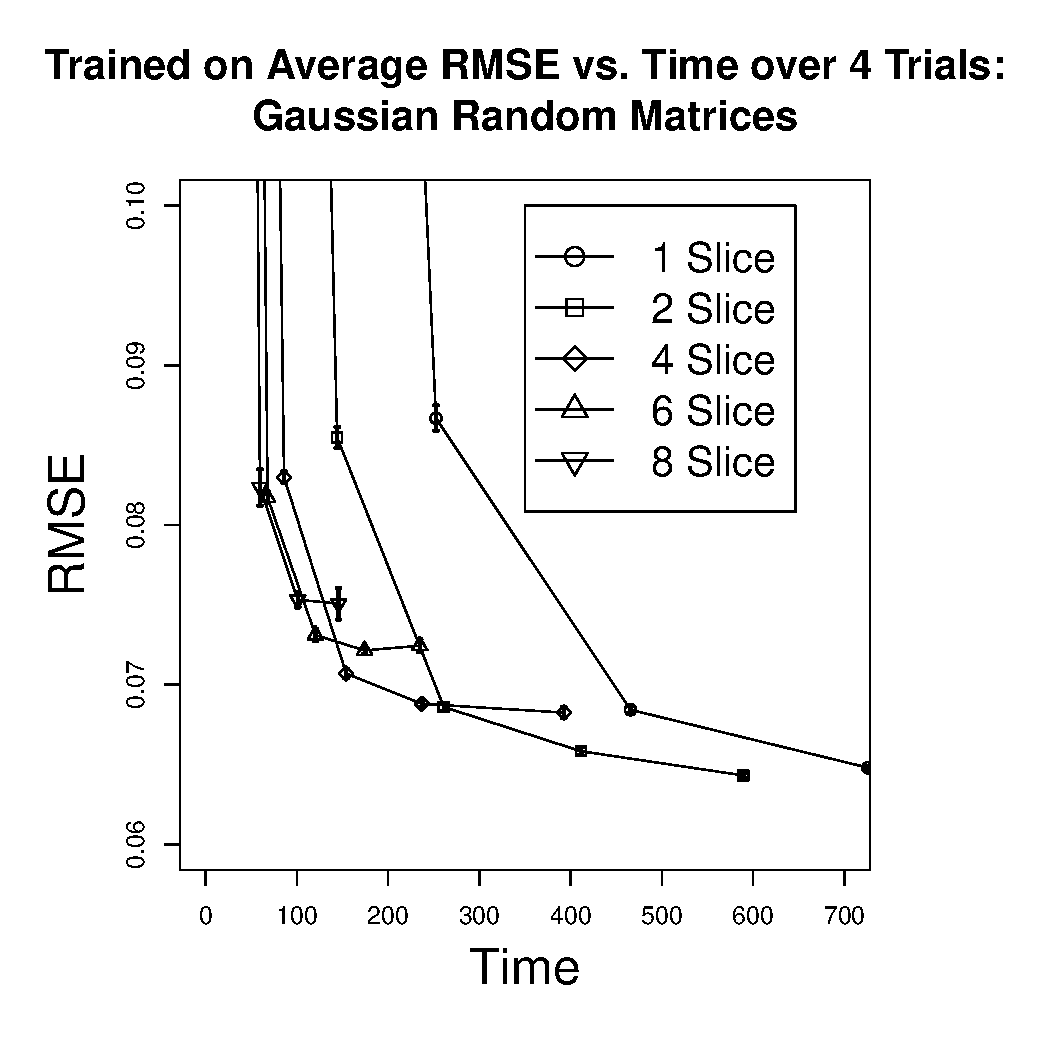
\includegraphics[width=\textwidth]{Graphs/4000_90_1_to_4_RvT_graph.pdf}}
		\caption{Training Data.}
\end{center}
	\end{subfigure}
\hspace{1cm}
	\begin{subfigure}[b]{.45\textwidth}
\begin{center}
		\fbox{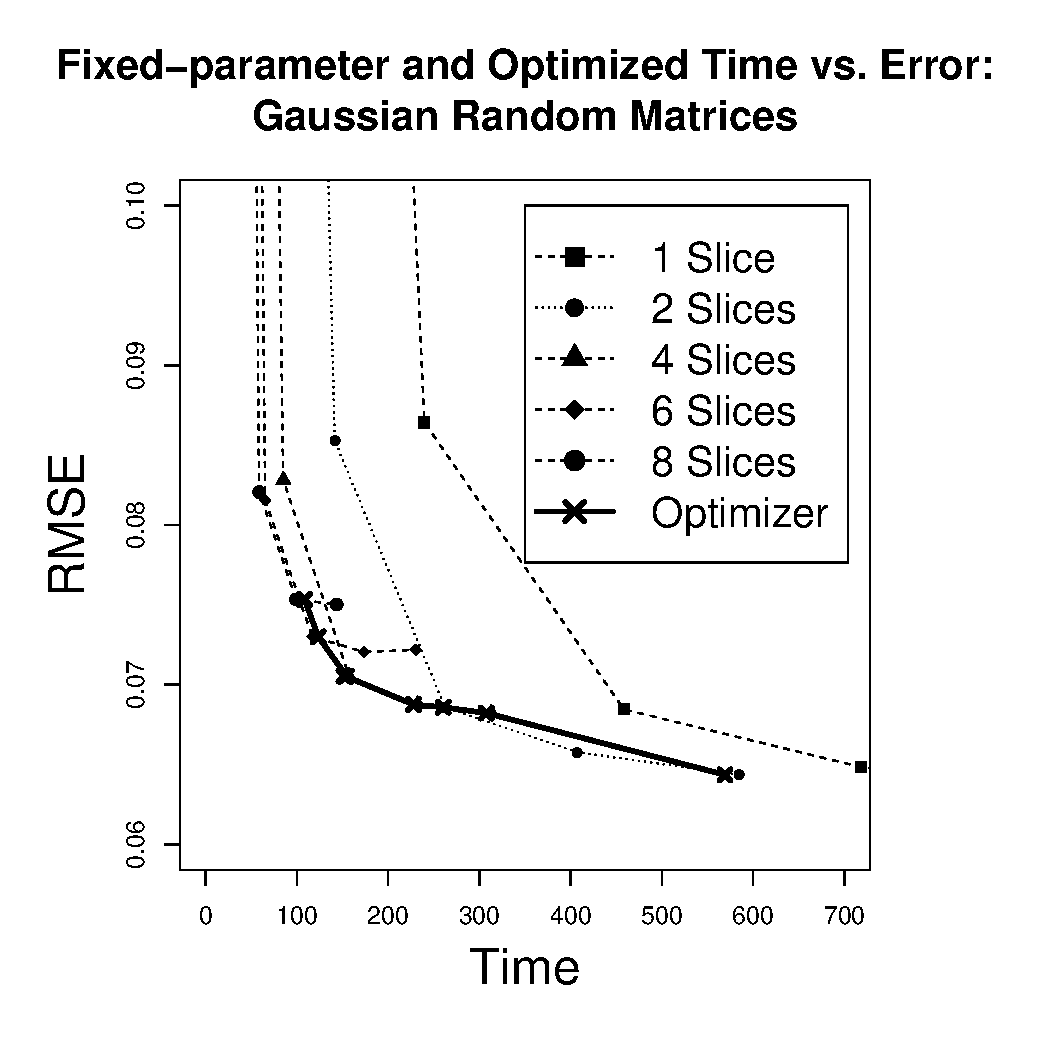
\includegraphics[width=\textwidth]{Graphs/Opt_Gaussian_4000.pdf}}
		\caption{Testing Data.}
\end{center}
	\end{subfigure}
\hfill
	\caption{Plots of vs. Time Error taken to factor a 4000 by 4000 
	low-rank matrix drawn from a Gaussian distribution. The choices of the 
	optimizer are indicated in the testing plot.}	

\end{figure*}

\subsection{Movielens Data}
The second dataset we used to test the optimizer was the Movielens10M 
dataset. The Movielens dataset is a set of entries 
$(\text{UserID},\text{MovieID},\text{rating})$, with the rating 
parameter being a half-integer between $1$ and $5$. One can think of 
these tuples as specifying the entries of a matrix with rows 
and columns indexed by users and movies. 

The reason we might want to find a low-rank completion of this matrix 
is the assumption that there are a small number of properties that 
influence the way people rate movies. Then the two factors tell you 
how a person values each property, and how each movie is correlated 
with these properties. This lets you make predictions even on the 
hidden entries of the matrix, i.e. the movies a user has yet to 
see or rate. 

There are some qualitative differences between this data and the 
synthetic data in the previous section. The entries come from 
the range $[1,5]$ rather than being concentrated around zero, 
and thus the RMSE's for this section are much larger. The 
Gaussian matrices also come from a well-understood distribution; this
means we can make theoretical guarantees about the behavior of  DFC 
on these instances, and also that it behaves pretty consistently across 
different random matrices. In the Movieens10M set we have no such 
guarantee, but under the assumption that the order of people is randomized,
we can hope that Movielens users behave similarly across partitions. 

The dataset was partitioned by the UserID into seven different 
pieces and the pieces were grouped to form the training/testing 
splits mentioned in the first section. Figure \ref{fig:movietraintest} 
displays the optimizer's performance on one of these splits. As before, 
each curve represents one of the choices of the division parameter in DFC. 
Once again we observe the intersection points where the division 
parameter should be changed for optimality to be satisfied. The bold 
line represents the optimized parameters for each budget. The graphs 
here are qualitatively the same as the graphs from the previous section. 
For every time budget, the optimizer picks the best division parameter. 

Table \ref{fig:MovieCrossTable} summarizes the results of each of the 
training/testing splits for the Movielens dataset. Averaged over 
all these splits, the optimized parameter choices perform within 
$2\%$ over the minimal error, and coming 
within $3\%$ over the budget.

\begin{table}
\label{fig:MovieCrossTable}
\begin{center}
    \begin{tabular}{| p{2.2cm} | p{2.2cm} | p{2.2cm} |}
    \hline
    Testing Set & \% Over Optimal Error & \% Over Time Budget \\ \hline
    1 & 2.0\% & -11.9\% \\ \hline
    2 & 0.1\% & -10.9\% \\ \hline
    3 & -1.8\% & -10.2\% \\ \hline
    4 & -1.0\% & -9.3\% \\ \hline
    5 & 1.1\% & -10.5\% \\ \hline
    6 & 0.9\% & -14.9\% \\ \hline
    7 & -2.9\% & 2.3\% \\ \hline
    \end{tabular}
\end{center}
\caption{Average regret and time for k-fold cross-validation of optimizer run on the seven Movielens matrices. Percentages are in relationship to best possible error and time budget respectively.}
\end{table}

\begin{figure*}
\label{fig:movietraintest}
	\begin{subfigure}[b]{.45\textwidth}
\begin{center}
		\fbox{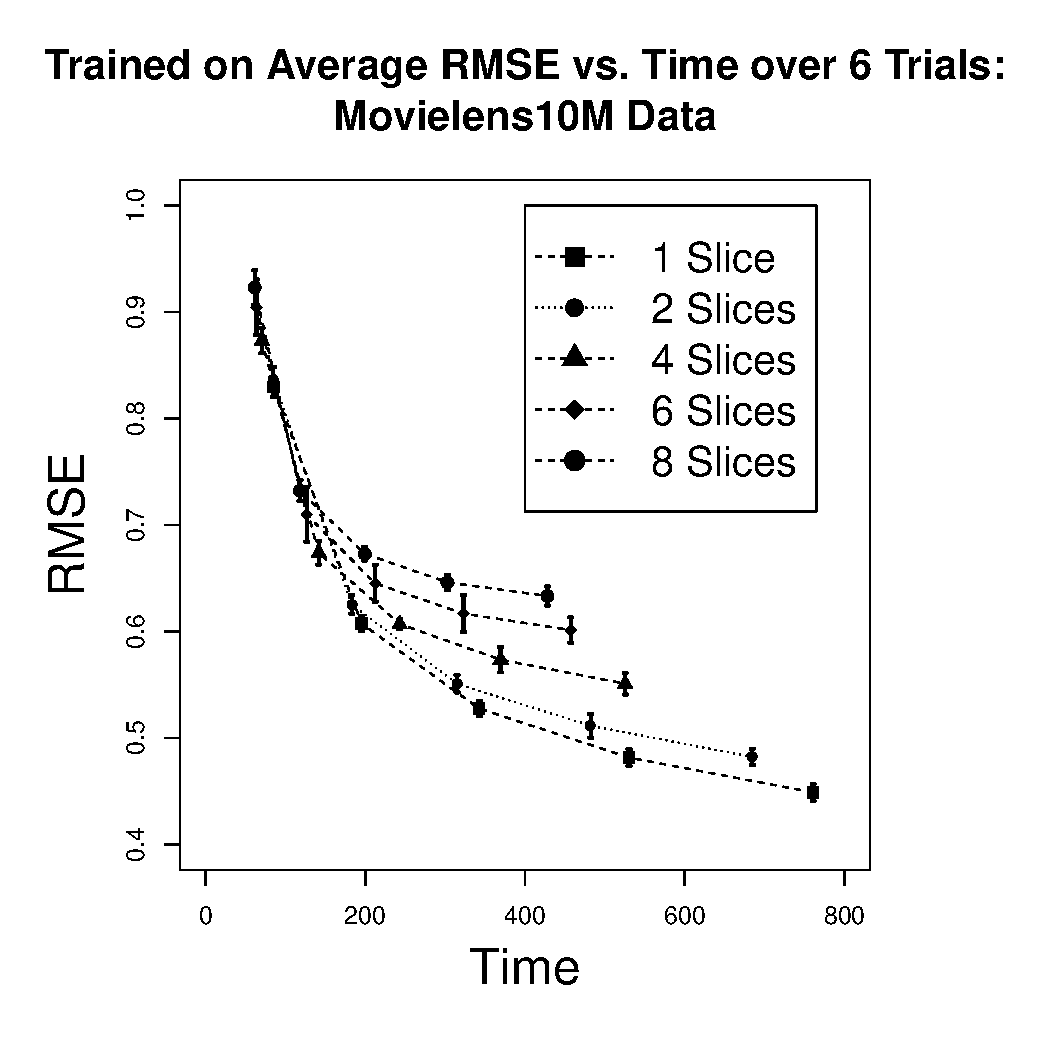
\includegraphics[width=\textwidth]{Graphs/movielens10M_1_to_4_RvT_graph.pdf}}
		\caption{Training Data.}
\end{center}
	\end{subfigure}
\hspace{1cm}
	\begin{subfigure}[b]{.45\textwidth}
\begin{center}
		\fbox{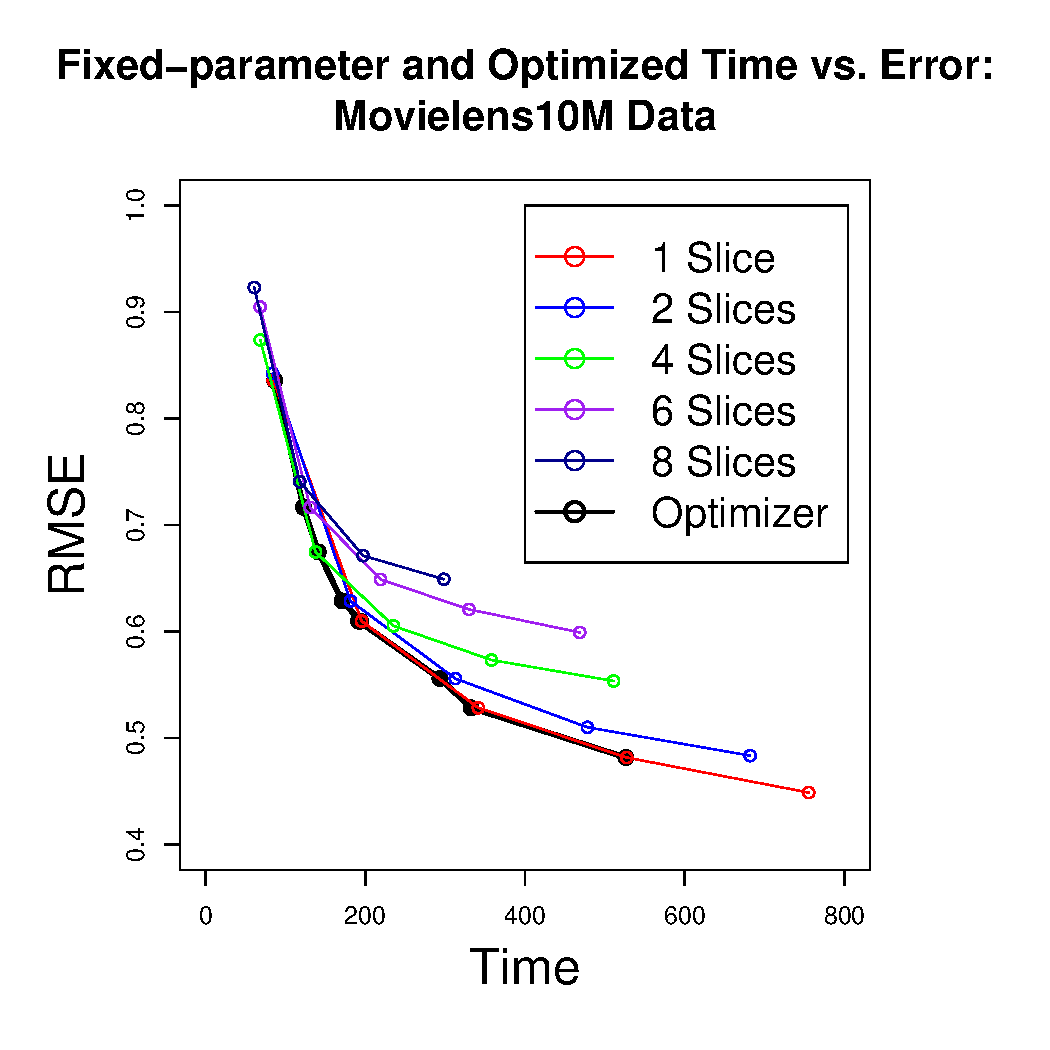
\includegraphics[width=\textwidth]{Graphs/Opt_movielens.pdf}}
		\caption{Testing Data. }
\end{center}
	\end{subfigure}
\hfill
	\caption{Plots of Time vs. Error taken to factor the Movielens10M 
	Dataset partitions. The optimizer's choices are shown on the testing
	plot.}	

\end{figure*}

\subsection{Training with Limited Data}
In an effort to discover how much training data we need for accurate 
optimizer predictions, we also ran some tests on training/testing 
splits with smaller training sets. Instead of training on six 
data partitions, we tried training the optimizer on only two partitions 
and testing it on the remaining five. The optimizer performs basically 
as well as if we had trained on almost all the partitions. 
Table \ref{fig:MovieTrain2Table} summarizes these results. We believe 
this is because the data is qualitatively the same across all the 
partitions, so the additional partitions do not add a lot of information 
to the optimizer. Distributions with higher variance in behavior 
may require significantly more learning, though we have not yet 
tested this. 

\begin{table}
\label{fig:MovieTrain2Table}
\begin{center}
    \begin{tabular}{| p{2.2cm} | p{2.2cm} | p{2.2cm} |}
    \hline
    Testing Set & \% Over Optimal Error & \% Over Time Budget \\ \hline
    1 & -1.8\% & -10.5\% \\ \hline
    2 & -1.1\% & -11.7\% \\ \hline
    3 & 1.1\% & -12.0\% \\ \hline
    4 & 0.02\% & -13.9\% \\ \hline
    5 & -2.9\% & 2.29\% \\ \hline
    \end{tabular}
\end{center}
\caption{Average pecent regret and time for k-fold cross-validation of optimizer run on the seven Movielens matrices. Percentages are in relationship to best possible error and time budget respectively.}
\end{table}


\subsection{Testing Explore and Estimation Modes}
\label{sec:estEval}
The previous sections show that our optimizer performs quite well 
when the training set accurately reflects the behavior of the algorithm 
on the parameter space of future jobs. However, sometimes an 
application can receive an instance that is unlike the previously 
seen jobs. For example, a matrix from the same distribution with more
revealed entries could take more time to process (this is a realistic
example for recommender systems, in which the users add more and more
ratings to the system). In this case, we want to estimate  the computational
costs in the unknown regions of the parameter space, and to use some 
randomness while picking our parameters so that we can adjust our estimates
about the parameter space to reflect reality. 
Ideally, the optimizer will complete the estimate and explore phase 
without sacrificing too much in the error or time of the computation, 
so we pick parameters proportionally to the error we expect to get 
with those settings. 

We tested this functionality in the setting where the size of the problem
instance changes. To do this, we gave the optimizer training data from 
$2000 \times 2000$ Gaussian random matrices, and applied our estimation 
mode to guess runtime profiles for $4000 \times 4000$ Gaussian 
random matrices. Then, we gave the optimizer a sequence of 
ten $4000 \times 4000$ Gaussian random matrices and asked the 
computation to finish within 200 seconds. While exploring, 
the optimizer was able to find a parameter setting with an error 
that was within $15\%$ of the best parameter choice that satisfies 
that budget that we could find in hindsight. It did not find better 
settings because we over-estimated the amount of time per iteration, 
and so the optimizer did not try running with more iterations because 
it thought that would violate the budget. This is a problem that could be
much improved with better models for time per iteration, as discussed
in the conclusion.

\begin{table*}
\label{fig:4kAdaptiveTable}
\begin{center}
    \begin{tabular}{| p{2.2cm} | p{2.2cm} | p{2.2cm} | p{2.2cm} | p{2.2cm} |}
    \hline
    Test Matrix & RMSE & Running Time (sec) & Slices & Iterations \\ \hline
    1 & 0.26 & 41.7 & 4 & 10 \\ \hline
    2 & 0.27 & 37.0 & 5 & 10 \\ \hline
    3 & 0.08 & 67.7 & 6 & 20 \\ \hline
    4 & 0.08 & 74.8 & 5 & 20 \\ \hline
    5 & 0.26 & 70.0 & 2 & 10 \\ \hline
    6 & 0.09 & 239 & 1 & 20 \\ \hline
    7 & 0.26 & 124 & 1 & 10 \\ \hline
    8 & 0.26 & 50.8 & 3 & 10 \\ \hline
    9 & 0.27 & 33.7 & 7 & 10 \\ \hline
    10 & 0.09 & 140 & 2 & 20 \\ \hline
    \end{tabular}
\end{center}
\caption{Parameter choices and results for running the optimizer in explore and estimation modes on ten Gaussian random 4000 by 4000 matrices, using
data from 2000 by 2000 Gaussian matrices.}
\end{table*}


\section{Related Work}
There has been a large amount of work on automatic parameter choice, 
especially for regularization parameters in various regression algorithms 
\cite{CI12},\cite{GEE10},\cite{BBGH07}. However, many of these results depend on assuming some 
underlying structure in the data, and exploiting that in order to provide 
analytic techniques that compute the optimal or near-optimal choice of 
parameter. Many of these automatic tuning algorithms are also extremely 
application-specific. 

To our knowledge, there is no general framework for automating parameter 
choice that can be applied independent of algorithm or task. In this work 
we propose a system to optimize parameters that depends only on the input 
and output of the algorithm. Our system does not assume any underlying 
data model, and only uses its own history to estimate optimal parameters. 
This approach may give worse results than the model approach if the model 
is carefully chosen, but this is not always possible, and it does not
allow for changes to the data over time.

\section{Conclusions}
We have designed and implemented an optimizer for distributed matrix 
computation. 


%ACKNOWLEDGMENTS are optional
\section{Acknowledgments}

%
% The following two commands are all you need in the
% initial runs of your .tex file to
% produce the bibliography for the citations in your paper.
\bibliographystyle{abbrv}
\bibliography{sigproc}  % sigproc.bib is the name of the Bibliography in this case
% You must have a proper ".bib" file
%  and remember to run:
% latex bibtex latex latex
% to resolve all references
%
% ACM needs 'a single self-contained file'!
%
%APPENDICES are optional
%\balancecolumns

\balancecolumns
% That's all folks!
\end{document}
